\section{BioMérieux Solution}

\begin{figure}[h]
    \centering
    
\includegraphics[scale=0.5]{img/bmx.png}
    \caption{Logo de BioMérieux}
\end{figure}

BioMérieux est une entreprise spécialisée dans le diagnostic in vitro et dans la microbiologie.
Cette entreprise conçoit et fabrique des instruments permettant de diagnostiquer des maladies et de faire des analyses microbiologiques.
BioMérieux dispose d'un showroom permettant de montrer leurs produits à leurs futurs clients.

\subsection{Situation initiale}

Dans ce Showroom, un ensemble de dispositifs interactifs sont mis en place pour présenter les produits et l'entreprise.
Parmi ces équipements, on retrouve l'espace solution.
Cet espace présente un exemplaire physique des principales machines conçues par BioMérieux.
Un projecteur permet alors d'afficher une image sur une vitre opacifiante, cette image projetée est l'écran d'un Mac mini disposé dans la salle technique du Showroom;
On utilise un lidar\footnote{Le lidar est un laser rotatif permettant, par balayage, de détecter la position d'un élément dans l'espace.} Pour repérer l'emplacement du doigt sur la vitre et ainsi contrôler l'ordinateur.

L'application présente avant ma mission était développée en C++ avec OpenFrameworks\footnote{OpenFrameworks est un framework se basant sur de nombreuses librairies permettant la création simplifiée d'applications graphiquement poussées. Il est très utilisé dans le domaine de la scénographie et du creative coding.}.
Cette application présente un arbre de composants graphiques chacun affichant un élément de l'interface.
Ce système, bien que fonctionnel, est assez peu flexible au regard des nouvelles fonctionnalités demandées par BioMérieux.

En effet, BioMérieux à récemment changé son logo et sa charte graphique pour un aspect plus épuré et flat-design\footnote{Le flat-design est un courant de design moderne qui possède une approche minimaliste de l'interface en se basant sur des aplats de couleurs unis et des effets d'ombres.}.
Pour refléter ce changement dans leur showroom, l'entreprise a demandé un redesign de l'application.
De plus, pour pouvoir gérer par eux même les produits présents dans l'application, BioMérieux a demandé la mise en place d'un back-office qui permettra d'éditer le contenu de l'application sans faire appel à LTBL .

\begin{figure}[h]
    \centering
    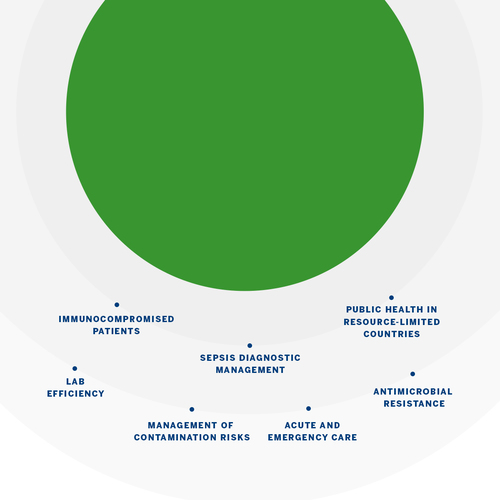
\includegraphics[scale=0.195]{img/resized-bmx-1-new.jpg}
    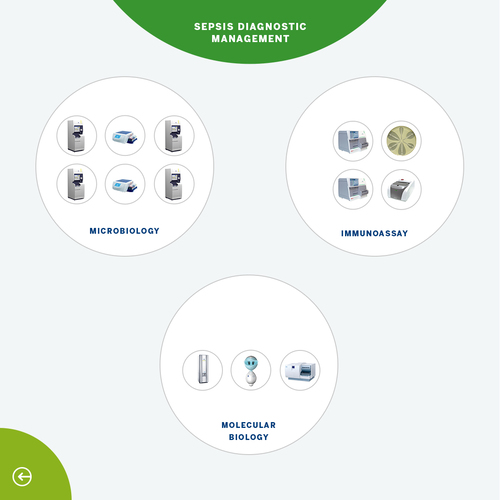
\includegraphics[scale=0.195]{img/resized-bmx-2-new.jpg}
    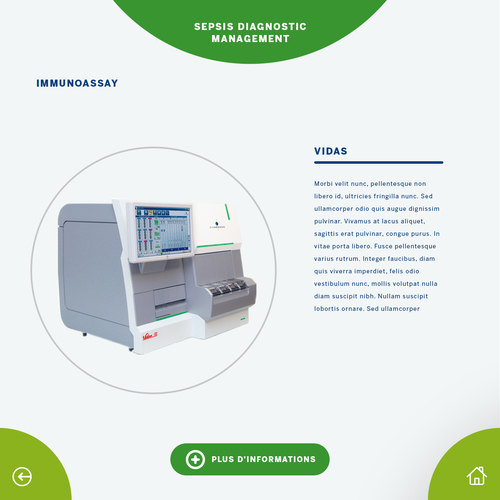
\includegraphics[scale=0.195]{img/resized-bmx-3-new.jpg}
    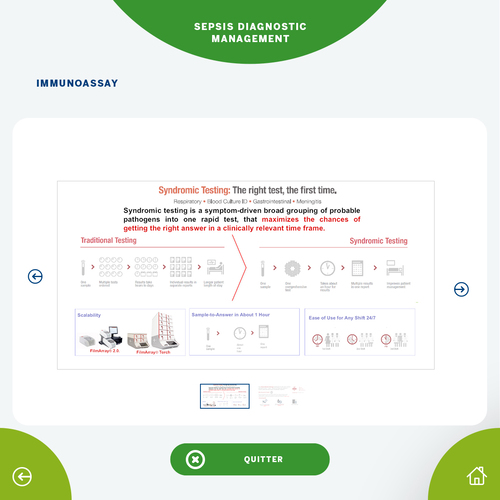
\includegraphics[scale=0.195]{img/resized-bmx-4-new.jpg}
    \caption{Design renouvelé de l'application Biomérieux}
\end{figure}

Enfin, dans une optique de recherche et développement d'une solution universelle de back-office chez LTBL il fallait aussi réfléchir à un système flexible de stockage de données.

\clearpage

Pour résumer, les fonctionnalités demandées sont :

\begin{itemize}
    \item La mise à jour de la charte graphique de BioMérieux
    \item La mise en place d'un back-office pour gérer les produits
    \item Faire en sorte que le back-office puisse être réutilisé dans d'autres projets LTBL
\end{itemize}


\subsection{Conception de la solution}

Le code précédent étant produit en C++, il est peu adaptable au redesign et à l'implémentation d'un backoffice utilisable par le client.
De plus, les données sont directement intégrées dans le code et il serait chronophage et peu rentable de modifier cette application pour qu'elle s'adapte aux nouveaux besoins.
J'ai donc décidé de reprendre l'application depuis le début et de choisir une solution technique qui me semble plus adaptée à une interface.

Pour ce projet, j'ai utilisé \emph{Electron} qui permet de créer des interfaces facilement à l'aide des technologies Web.

Pour le stockage des données, j'ai opté pour une base de données \emph{SQLite} permettant un stockage dans un fichier sans serveur superflu.
En effet, SQLite est une librairie C mettant à disposition un langage SQL et un stockage de données dans un fichier.
Cette technique est très intéressante dans notre cas, car les données ne seront qu'utilisées par l'application.
De plus, l'application ne nécessite pas de grandes performances et donc pas d'optimisation particulière que peuvent présenter les serveurs SGBDR\footnote{Système de Gestion de Bases de Données relationnelles} comme MariaDB ou PostgreSQL\@.

Enfin, pour gérer ces données j'utilise \emph{Sequelize}, un ORM JavaScript permettant de communiquer avec la base de données.
Cette librairie permet de représenter les données sous forme d'objets JavaScript pour éviter d'écrire les requêtes à la main et ainsi avoir une meilleure intégration des données dans l'environnement JavaScript.

\subsubsection{Electron}

Pour développer l'application, j'ai décidé d'utiliser Electron.

\begin{figure}[h]
    \centering
    
\includegraphics[scale=0.2]{img/electron.png}
    \caption{Logo d’Electron}
\end{figure}

Electron est un framework permettant de concevoir des applications natives en utilisant les technologies web.
Il embarque le moteur de rendu et le moteur JavaScript de Chromium, mais ajoute les fonctionnalités de NodeJS permettant d'interagir avec le système hôte.
Chromium est l'un des navigateurs les plus avancés dans l'intégration des nouvelles normes et cela permet de profiter de nouvelles fonctionnalités très intéressantes comme les WebComponents et WebGL .
Enfin, on peut toujours accéder au système de fichiers de l'utilisateur et faire de la dépendance de modules NodeJS avec les fonctionnalités que propose Electron en plus des fonctionnalités de base que l'on retrouve sur un site web classique.

L'utilisation de ce framework est intéressante dans le cas de cette application, car elle permet de concevoir des interfaces simplement.
Les langages web sont spécifiquement dédiés à la création d'interfaces comme le demande notre projet.
Ainsi, on peut estimer que recoder l'application avec un nouveau design et les nouvelles fonctionnalités prendraient moins de temps que d'adapter l'ancienne application.

\subsubsection{WebComponents}
\label{webcomponents}

Le système de WebComponents est un ensemble de nouvelles normes mises en place il y a peu de temps par le W3C et implémentées dans Chromium permettant de créer de nouveaux tags HTML avec des fonctionnalités spécifiques et isolées du reste de l'architecture de la page.

\clearpage

Un WebComponent est basé sur 4 normes :

\paragraph{Custom Elements} Une fonctionnalité permettant de créer un tag HTML personnalisé et reconnu par le navigateur comme faisant référence au code associé sous forme de classe.

\paragraph{HTML Template} Le tag \texttt{<template>} permet de créer un élément qui ne sera pas visible par l'utilisateur, mais qui servira de squelette pour la création de futurs éléments.
Dans les WebComponents, on les utilise pour créer le squelette de base de notre \component.

\paragraph{Shadow DOM} Un concept permettant d'isoler une partie de l'arborescence d'une page Web.
Cela implique l'isolation du style et des éléments.
Cette technologie sert à créer le contenu caché de notre futur élément qui apparaîtra comme une blackbox\footnote{Une blackbox est un concept dans lequel on cache le fonctionnement interne d'un élément pour ne mettre à disposition du développeur uniquement la partie haut niveau.}.

\paragraph{HTML Import} Permet d'importer un fichier HTML externe.
Cela permet notamment d'inclure tout le code HTML, CSS et JS d'un \component dans un même fichier HTML .
Il suffira ensuite d'importer cet unique fichier pour pouvoir utiliser le \component.

\bigskip

Le développement en WebComponents présente de nombreux avantages.
L'isolation du style CSS dans le Shadow DOM permet de ne pas provoquer de conflit CSS lors d'une sélection un peu trop générale sur le fichier de style de base.
L'isolation du JavaScript permet de se concentrer uniquement sur le \component interférer avec le reste de l'application.
Enfin, l'approche unitaire des WebComponents permet une réusabilitié importante.

Mais l'approche par \component pose aussi des difficultés.
En effet, il faut penser le \component en tant qu'élément générique.
Si on fait un \component trop spécifique ou dépendant de ses voisins, il sera difficile de réutiliser le \component dans un autre contexte que celui pour lequel il était prévu au début.
Cela implique de réfléchir à la structure de l'application en amont.
Et il ne faut plus penser l'application dans son ensemble, mais comme un ensemble de blocs réutilisables ajoutés les uns aux autres.

Faire un bloc réutilisable passe par l'utilisation des attributs HTML comme vecteurs de transmission d'informations.
Mais aussi l'utilisation d'événements JavaScript comme vecteur de signal pour avertir les parents.

\bigskip

Dans ce projet, j'ai été amené à découvrir cette nouvelle norme du W3C par le biais des employés de l'entreprise qui utilisaient déjà cette technologie.
J'ai découvert les WebComponents et ai expérimenté avec ceux-ci durant ce projet.
J'ai eu l'occasion, par la suite, d'affiner mes connaissances sur le sujet dans le cadre des 5 autres projets qui les utilisent.

\subsection{Structure}

Pour cette structure, j'ai puisé dans mes connaissances acquises durant ma formation pour concevoir un système en 3 blocs.

\begin{figure}[h]
    \centering
    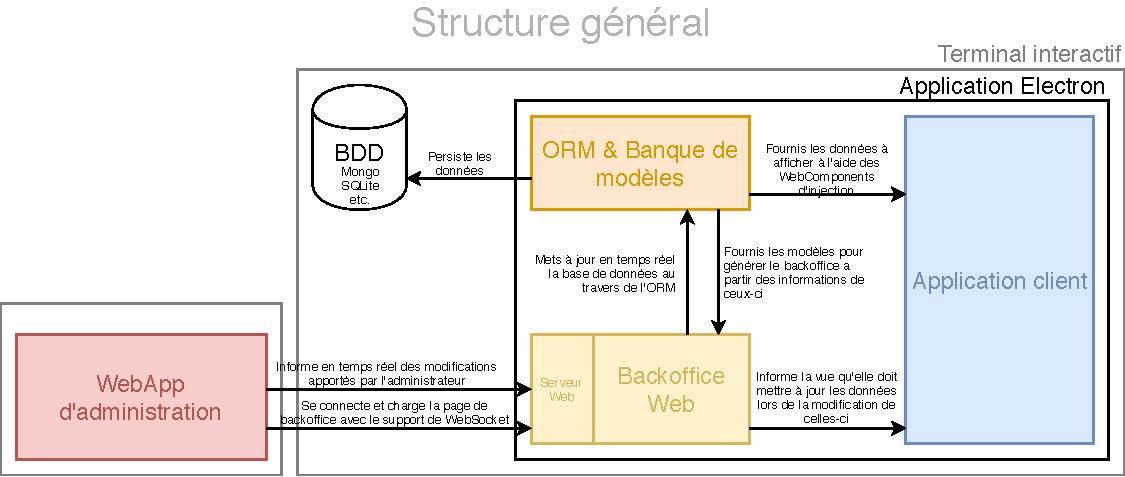
\includegraphics[scale=0.6]{img/Proposition-utopia.pdf}
    \caption{Structure générale de l'application Biomérieux}
\end{figure}

\subsubsection{Modèle}

Le modèle est la partie de l'application qui définit l'organisation et le stockage des données requis par les éléments de l'interface.

Pour définir et stocker les données, j'utilise la librairie d'ORM\footnote{Un ORM est une librairie apportant une couche d'abstraction aux requêtes SQL par l'utilisation des fonctionnalités orientées objet du langage dans lequel elle est implémentée (ex : Doctrine en PHP, Sequelize en JavaScript, Django ORM en Python, etc.)} \emph{Sequelize}.
Elle a pour avantage d'être compatible avec la majeure partie des bases de données relationnelles les plus connues comme MySql, PostgreSQl, SQLite, etc.
Dans cet ORM, on doit définir un modèle, ce modèle sera utilisé pour créer les tables de la base de données.
J'ai décidé de définir ce modèle dans un unique fichier \texttt{model.js} permettant de centraliser leurs déclarations pour facilement les adapter en cas de changement d'avis du client.

L'objectif de cette structure est d'être le plus flexible possible pour pouvoir reprendre le même code dans un tout autre système.

\bigskip

Dans le cas de cette application pour BioMérieux, j'ai décidé de découper les données en cinq entités.
Ces entités représentent une table dans la base de données et permettent de faire le lien entre cette table et le code de l'application.
Pour construire ce modèle de données, je me suis basé sur les designs de l'application faits par le graphiste et des informations données par mon maître de stage.
L'une des difficultés ici fut de ne pas avoir de cahier des charges défini, ce qui m’a obligé à reprendre mon modèle plusieurs fois.
Mais la grande flexibilité du système m'a permis de continuer à développer sans me soucier de ces changements.

\bigskip

\begin{figure}[h]
    \centering
    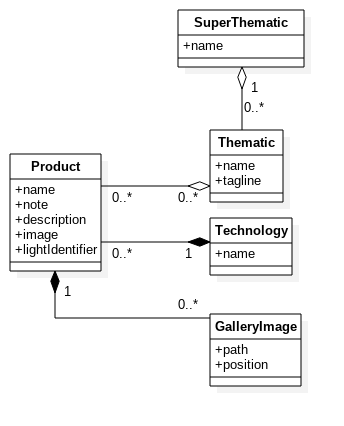
\includegraphics[scale=0.6]{img/uml-bmx-solution.png}
    \caption{Le diagramme UML du modèle de données de l'application BioMérieux Solutions}
\end{figure}

\clearpage

J'ai donc mis en place les entités suivantes

\paragraph{Produit} L'entité représentant un produit de Biomérieux.
Il contient un \emph{nom}, une \emph{description} en texte riche\footnote{Un texte riche est un ou plusieurs paragraphes formatés suivant une certaine syntaxe; on peut donc y ajouter des passages en gras, italique, insérés des images et des listes}, une \emph{image} uploadée, d'un \emph{identifiant de lampe} permettant d'envoyer des commandes OSC\footnote{Le protocole OSC (Open Sound Control) permet d'envoyer des commandes dans des paquets UDP au travers du réseau; il est très utilisé dans la scénographie pour faire communiquer les différents éléments de l'espace comme des lampes, des moteurs, etc.} Et d'une image de présentation.

\paragraph{Technology} Une technologie de produit, permettant de classifier les produits.
Un même produit est associé à une seule technologie.
Une technologie ne contient qu'un \emph{nom}.

\paragraph{Thematic} Une thématique permet de regrouper les produits en diverses catégories.
Il est ainsi possible d'ajouter un même produit à plusieurs thématiques.
Une thématique permet de classifier les produits dans divers domaines d'expertise.
Une thématique possède un \emph{nom} et une \emph{tagline} représentant le slogan de cette thématique.
Chaque thématique peut contenir plusieurs produits et un même produit peut se retrouver dans plusieurs catégories.

\paragraph{SuperThematic} Une thématique contenant plusieurs sous-thématiques.
J'ai choisi de créer une super thématique au lieu de faire une arborescence de thématique, car le client ne dit pas vouloir une arborescence plus grande que deux niveaux.
Mais aussi qu'il ne faut pas pouvoir ajouter des produits dans les super thématiques.
Une super thématique ne contient qu'un \emph{nom} tout comme les thématiques, mais peut contenir plusieurs thématiques.

\paragraph{GalleryImage} Chaque produit dispose de plusieurs images disposées dans une galerie consultable par l'utilisateur.
Cette entité permet alors de créer une image de cette galerie.
Un produit peut contenir plusieurs images et chaque image dispose d'un \emph{chemin} vers l'image uploadée et d'une \emph{position} dans la galerie représentée par un nombre.
Les images sont alors triées dans l'ordre de ce champ.

\subsubsection{Back-office}

Un Back-office est une interface simplifiée permettant au client final d'éditer le contenu de l'application sans l'intervention des créateurs.
Cela peut passer par un logiciel compagnon ou une interface Web.
Dans mon cas, j'ai choisi la deuxième option pour éviter de demander le développement et l'installation d'une deuxième, application.

Le Back-office est un serveur web exécuté au sein de l'application Electron.
Ce serveur web se base sur le modèle pour créer les formulaires de saisie des données.
Le back-office ne présente aucun code spécifique au modèle de BioMérieux, mais met en place une arborescence de formulaires générés en fonction du modèle défini par le développeur.
Cette technique permet de réutiliser ce back-office dans un tout autre contexte, mais permet aussi de changer le modèle sans difficulté.

Pour ce back-office j'ai utilisé \emph{Express} une librairie permettant de créer des applications Web très simplement et le moteur de template \emph{twig} que j'ai déjà utilisé dans le projet Web de l'eXia.

\bigskip

Avec le recul de mon stage, je me rends compte que le développement d'une application compagnon aurait été plus intéressant pour éviter qu'un pirate ayant accès au réseau de l'application puisse librement en modifier le contenu.
De plus, cela aurait permis d'améliorer les performances en évitant de démarrer un serveur web à chaque utilisation de l'interface client.

Mais, l'approche que j'ai utilisée permet une plus grande simplicité d'opération par la mise à jour en direct de la vue client et l'absence de fichier à transférer.

\subsubsection{Affichage client}

 L'affichage client représente tout ce qui va être affiché par l'application Electron sur le terminal.
Cet affichage est le seul qui sera vu par les visiteurs du showroom.
Dans l'architecture utilisée, c'est la seule partie spécifique.
Dans cette partie, on utilise les WebComponents (\emph{cf} partie \ref{webcomponents}) pour concevoir l'application.

Parmi ces WebComponents, j'en ai créé des génériques permettant d'effectuer des tâches de base.


\paragraph{DataElement} Le plus important de ces WebComponents, car il permet, en tout point de l'application, de récupérer des données depuis la base de données et d'être averti quand ces données changent.
Cela permet de récupérer les données, mais aussi d'actualiser la vue en direct dès la modification de ceux-ci.
Cela est rendu possible par deux processus :
\begin{description}
    \item[Hooks Sequelize] Les entités sequelize disposent de Hooks permettant d'appeler une fonction lors d'action spécifique comme la création, la suppression ou la mise à jour de l'entité. J'utilise ces Hooks pour alerter le \texttt{<data-element>} de la modification des données.
    \item[IPC Electron] Electron, tout comme Chromium, est un logiciel multi processus. Le processus initial se charge de démarrer un processus enfant pour afficher les données. Ce processus initial est aussi en charge de la mise en route du back-office. Pour que les modifications soient effectuées dans tous les processus, j'envoie un signal IPC contenant l'entité modifiée pour qu'elle soit mise à jour dans tous les processus.
\end{description}

\paragraph{PageRouter} L'élément \texttt{<page-router>} permet de simuler le fonctionnement d'un système multi page.
Chaque élément placé dans ce WebComponents dispose d'un attribut \texttt{route} définissant l'URL de la page.
Une route peut contenir n'importe quel caractère, mais aussi des attributs en faisant précéder le nom du paramètre par des \texttt{:}.
On peut alors choisir la page à afficher en entrant l'URL de celle-ci dans l'attribut \texttt{page} du WebComponents \texttt{<page-router>}.

\paragraph{AnimationBlock} Un WebComponents d'animation se basant sur les modules d'animation de AngularJs ou de VueJs.
Il permet d'animer les éléments de l'interface à la fin de la production de l'application et de manière flexible.
Il se base sur les transitions CSS pour de grandes performances et ne s'active que lors du focus sur l'application.
J'en parle plus en détails dans la partie \ref{animationblock}.

\subsection{Installation}
\label{bmxinstallation}

La première installation de l'application s'est déroulée le 7 février dans les locaux de BioMérieux.
J'ai pu y découvrir le nouveau bâtiment de l'entreprise et son showroom très impressionnant.

Le dispositif est disposé sur une vitre opacifiante et le dispositif de pointage (autrefois un lidar) est remplacé par une caméra infrarouge et un stylo spécifique.
Ce système permet une précision de pointage plus importante et un système plus discret.

Malheureusement, en raison d'un problème touchant l'ensemble du showroom, je n'ai pas eu l'occasion de tester l'application en condition réelle.
Mai j'ai tout de même pu soumettre mon application à l'utilisateur final qui semble intéressé par les nouvelles fonctionnalités.

Une nouvelle installation est planifiée pour le 12 avril pour installer mon application dans le showroom et démarrer les premiers tests en conditions réelles.

\subsection{Conclusion}
\label{bmxconclusion}

Ce projet fut le premier au sein de l'entreprise LTBL .
J'ai eu l'occasion de ma familiariser avec les services, l'équipe de développement et de design et de découvrir les technologies utilisées en interne.

Ce projet fut mon premier projet utilisant les WebComponents, une technologie très utilisée chez LTBL.
En revanche, je me rends compte en fin de stage que j'ai fait des erreurs de structure dans mon découpage.
Ces erreurs ne peuvent malheureusement pas être corrigées dans le peu de temps qu'il me reste pour finir mon stage, mais me permettent de constater mon avancée dans cette nouvelle technologie.
